% !TeX program = xelatex
% Canonical manuscript entry point; compile from the repository root.
% Internal research draft, 2026-10-22. No measured performance claims.
% Official unmodified USENIX style is supplied alongside this file.
\documentclass[letterpaper,twocolumn,10pt]{article}
% Load hyperref before the XeLaTeX compatibility style.
\usepackage{hyperref}
\usepackage{usenix2019_v3_xetex}
\usepackage[T1]{fontenc}
\usepackage{amsmath,amssymb}
\usepackage{booktabs,array,tabularx}
\usepackage{graphicx}
\usepackage{tikz}
\usetikzlibrary{arrows.meta,positioning,fit,calc}
\usepackage{microtype}
\usepackage{xurl}
\hypersetup{breaklinks=true,hidelinks}
\newif\ifanonymouspreview
\ifdefined\AnonymousPreview\anonymouspreviewtrue\else\anonymouspreviewfalse\fi
\ifanonymouspreview
  \newcommand{\sysname}{System X}
  \hypersetup{pdftitle={System X: Internal Research Draft},pdfauthor={}}
\else
  \newcommand{\sysname}{BrewFS}
  \hypersetup{pdftitle={BrewFS: Delta-Based Multi-Agent Workspaces with Packed Metadata and Variable-Granularity Object Storage},pdfauthor={}}
\fi
\newcommand{\sys}{\sysname{} }
\newcommand{\code}[1]{\texttt{#1}}
\newcommand{\KiB}{\,\mathrm{KiB}}
\newcommand{\MiB}{\,\mathrm{MiB}}
\newcommand{\GiB}{\,\mathrm{GiB}}
\newcommand{\researchq}[1]{\textbf{RQ#1.}}
\newcolumntype{Y}{>{\raggedright\arraybackslash}X}
\pagestyle{plain}
\begin{document}
\title{\sysname: Delta-Based Multi-Agent Workspaces with Packed Metadata\\
and Variable-Granularity Object Storage}
\author{Internal research draft\\23 October 2026}
\date{}
\maketitle
\begin{abstract}
Coding agents need ordinary writable volumes, isolated views of shared
environments, and read-only access to published state. We present the design
of \sysname, an object-backed file system with three optional, composable
mechanisms. Delta-based workspaces resolve a shared immutable baseline and
private changes into a task's file-system view. Packed Metadata organizes
immutable directory entries, attributes, and data locators into indexed pages
on object storage; it can serve a workspace lower or a standalone read-only
mount. Variable-Granularity Object Storage separates client object formation
from optional backend encoding and verification layouts. A workspace can use
native metadata, a packed snapshot can operate without private changes, and
an ordinary volume can choose object granularity independently of both.
We explain their state, access, and publication rules, then distinguish
architectural composition from combinations supported by current mount paths.
A reanalysis of 1,138,884 FUSE requests from eight coding-agent task runs
characterizes metadata traffic, read/write sizes, and temporal heterogeneity.
The evaluation plan tests each mechanism and their legal combinations while
controlling caching, request coalescing, durability, and construction costs.
The workload observations do not establish system speedups.
\end{abstract}

\noindent\textbf{Status.} This is an author working document: design, source
audit, and measured passthrough workload observations are distinguished from
planned system experiments. Integration,
correctness, and performance claims require the evidence described below.

\section{Introduction}
\label{sec:intro}

Coding agents work through ordinary file-system tools: they traverse a
repository, inspect source files, edit code, and run builds and
tests~\cite{sweagent2024,openhands2025}. Consider a service that launches
several attempts from the same repository revision and dependency set.
Each attempt needs a consistent starting view and must be able to change
files independently. Making that starting state available is only the first
part of serving a task. Throughout execution, the file system must also
resolve names and attributes, locate file contents, and serve reads and writes.

Sharing a baseline addresses provisioning, but leaves these access costs
open. Layered namespaces and copy-on-write branches already let tasks reuse
state while keeping changes private~\cite{overlayfs,branchfs2026,deltafs2021}.
A shared directory tree still needs a metadata access path, and its files
still need a data access path. Immutable distribution systems support
indexed, demand-loaded state~\cite{cvmfs2011,nydus_rafs}; grouping records
can amortize requests, but may also fetch records a task never uses. On the
data path, larger objects can amortize object requests, while smaller
independently readable units can limit excess transfer and verification.
The problem is therefore to support independent task views while controlling
the work of provisioning state, obtaining metadata, and accessing file data.

Our observations motivate considering access throughout a task's lifetime.
We reanalyzed 1,138,884 FUSE requests from eight coding-agent task runs
(Section~\ref{sec:agent-observations}). Metadata operations, including
unsuccessful probes, made up more than half of the requests in each of the
two workload groups. Reads and writes had mixed request lengths, and
activity varied substantially across tasks and over time. A provisioning
mechanism alone leaves this metadata and data traffic to the underlying
storage path.

Our design separates the state a task shares from the units used to access
that state. A workspace needs an immutable baseline identity and rules for
resolving private changes; those rules need not prescribe the baseline's
metadata format. Immutable metadata can be organized for lookup and reuse
whether or not its consumer needs a writable workspace. Likewise, object
formation and backend read units can be selected without changing which
file version a task sees. These boundaries allow choices driven by state
reuse, metadata locality, and data access to remain distinct.

\sys realizes this design in an object-backed file system with three
mechanisms. \emph{Delta-Based Workspaces} resolve a shared immutable
baseline together with private namespace and data-mapping changes, avoiding
a separate materialized baseline for each task. \emph{Packed Metadata}
places immutable names, attributes, and data locators in indexed, bounded
groups on object storage so that readers can fetch and reuse related
records. \emph{Variable-Granularity Object Storage} lets deployments choose
client object size separately from optional encoding and verification
layouts on a compatible backend, to trade request count against transferred
bytes and processing work.

The mechanisms are optional and can be composed. A workspace can inherit
a native metadata layer; a packed snapshot can serve a read-only consumer;
and an ordinary writable volume can choose its object block size with the
backend's default layout. When tasks reuse a stable environment, multiple
workspaces can instead reference one packed baseline. This composition
shares the baseline's representation while preserving each task's private
changes; it does not make packing a prerequisite for workspace isolation.

The paper develops the state and access rules that make these choices
compatible: private-view resolution, immutable metadata lookup and
publication, and the mapping from file ranges to object and backend work
units. Section~\ref{sec:implementation} identifies the paths present in the
current code and their integration limits. The completed workload study
characterizes request structure; it does not establish cross-task sharing
or system speedups. Performance and failure experiments remain to be
completed under the evaluation plan in Section~\ref{sec:evaluation}.

\section{Background and Motivation}
\label{sec:motivation}

\subsection{Task views and reusable state}

A coding-agent workspace contains source files, dependencies, generated
artifacts, and temporary files. In the deployment considered here, multiple
attempts can start from a common repository revision and dependency set.
For example, two attempts may initially read the same \code{src/parser.py}.
If one edits or deletes that file, the other must continue to see its own
version. The shared starting state must therefore have a stable identity,
and each attempt's changes must remain private. This is a requirement on
the visible file tree, independent of where its metadata and bytes reside.

Reuse is conditional on the deployment. A stable dependency tree may serve
many attempts, whereas generated outputs may be replaced on every run.
A baseline can cover a selected subtree; it need not include the entire
working directory. The value of sharing depends on overlap between tasks,
the amount of private modification, and how long the baseline remains
useful. These properties determine whether sharing is appropriate; they
are distinct from the access behavior of an individual task.

\subsection{From file operations to storage work}

To read \code{src/parser.py}, a tool first needs the path resolved and the
file's data located. An object-backed file system keeps names, attributes,
and file-to-object mappings in its metadata path, and retrieves payloads
from caches or object storage. Metadata services can batch requests and
cache records~\cite{tablefs2013,indexfs2014}; immutable distributions can
also organize records for demand fetching~\cite{cvmfs2011,nydus_rafs}.
Resolving a shared file therefore does not imply either a network request
per metadata operation or a particular metadata representation.

The requested file range also differs from the storage work it induces.
Kernel caching and readahead affect which requests reach FUSE. The client
then maps those requests to stored objects and may fetch a range or an
entire object. Backend encoding and integrity checks can require access
to still different units~\cite{azureec2012,okapi2025}. Writes similarly
pass through buffering and object formation before publication. Thus a
small file request does not by itself determine transferred bytes,
verification work, or uploaded object size. The following observations
characterize one point in this path: requests received by FUSE handlers.

\subsection{Observed requests in real agent runs}
\label{sec:agent-observations}

\paragraph{Capture and scope.}
We reanalyzed eight SWE-bench Verified task runs~\cite{swebench2024}: five
Core and three Exploratory. All used DSH 0.1.5-rc.1 and the CCSwitch-configured
model \code{deepseek-v4-flash}. Exploratory runs used a broader
investigation/testing prompt and a 30-minute budget; all finished earlier.
Each base-commit checkout was mounted through \code{libfuse-fs}
\code{PassthroughFs} on Ubuntu 24.04 under WSL; \code{rfuse3}
\code{LoggingFileSystem} recorded actual FUSE handler requests.
Streaming reanalysis covered all 1,138,884 events: 217,129 Core and 921,755
Exploratory. Counts retain every status, 64 setup/canary requests before
agent startup, and teardown, including 24 requests after recorded run finish.
Group statistics weight requests equally, not tasks. Per-task counts and
source-validation details are in the companion workload record.

\begin{figure*}[!t]
\centering
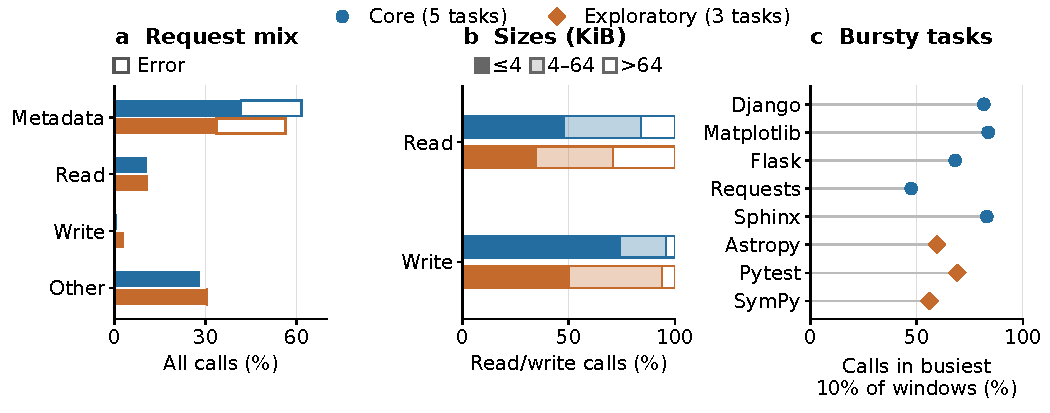
\includegraphics[width=\textwidth]{figures/agent-fuse/fuse-combined-compact.pdf}
\caption{Request structure across eight single-run FUSE captures.
Core bars precede Exploratory bars in each pair.
(a) Shares of all calls; white segments are errors within each total.
Metadata comprises \code{lookup}, \code{getattr}, \code{getxattr},
\code{readdirplus}, \code{opendir}, and \code{releasedir}; Other contains
every remaining method, including file open/flush/release.
(b) Each bar includes all reads or writes in its group. Dark, light, and white
segments denote $\leq4$, $(4,64]$, and $>64$ KiB, respectively
($1\,\mathrm{KiB}=1024$ bytes). Read counts are 22,142/98,292 and write
counts 1,112/23,600 (Core/Exploratory), all \code{ok}. Lengths are requested
FUSE bytes, not object sizes.
(c) Fraction of each task's calls in its busiest 10\% of one-second windows,
rounding the window count up; zero-call and final partial windows are retained.
All panels retain setup/teardown and every recorded status.}
\label{fig:agent-fuse-combined}
\end{figure*}

\paragraph{Metadata traffic and read dominance.}
The six metadata methods accounted for 61.5\% of Core and 56.4\%
of Exploratory calls (Figure~\ref{fig:agent-fuse-combined}a).
Restricting the denominator and numerator to \code{ok} events reduces these
shares to 52.0\% and 44.2\%: failed probes materially change the request mix.
Across tasks, the all-status share ranged from 39.6\% in SymPy to 65.4\% in
Django, so the group majority does not describe every task.
Read calls outnumbered writes by 19.9:1 in Core and 4.16:1 in Exploratory;
per-task ratios ranged from 3.12:1 (Pytest) to 42.7:1 (Matplotlib).
These observations motivate evaluating both positive and negative metadata
paths alongside data I/O.

\paragraph{A mixture of request sizes.}
Reads ranged from 4 to 128 KiB, with Core and Exploratory medians of 8 and
16 KiB. Writes ranged from one byte
to 128 KiB, with medians of 4,084 and 4,117 bytes, respectively.
Requests of at most 4 KiB accounted for 47.7\% and 34.5\% of reads, and
74.3\% and 49.9\% of writes. The interval $(4,64]$ KiB contained a further
36.2\% and 36.4\% of reads and 21.3\% and 44.0\% of writes
(Figure~\ref{fig:agent-fuse-combined}b).
This mixture motivates measuring how client fetching and uploads transform
requests before testing backend layouts. FUSE observations occur below kernel
caching and readahead; they do not identify application syscall sizes, unique
bytes, finalized object lengths, or an optimal block size.

\paragraph{Task and temporal heterogeneity.}
Tasks generated 8,542--634,726 calls. Astropy contributed 68.9\% of
Exploratory calls, versus 6.0\% for Pytest. Capture spans, from first to last
request start, were 42.7--71.3 seconds for Core and 119.9--556.1 seconds for
Exploratory. The busiest 10\% of one-second windows, rounded up per task,
contained 47.4--83.7\% of its calls (Figure~\ref{fig:agent-fuse-combined}c).
The companion record retains the full method breakdowns, size ECDFs,
and per-task cumulative time curves. Replay
should retain these per-task mixes and bursts. Each task was observed once;
different repositories, prompts, and budgets prevent a causal interpretation
of the group contrast. Without tool-phase labels, bursts cannot be assigned
to searching, editing, or testing.

\paragraph{Status semantics and evidence limits.}
The capture contained 872,519 \code{ok}, 253,669 \code{error}, and 12,696
\code{incomplete} events. Errors occurred in \code{lookup} (233,452),
\code{getxattr} (20,203), and \code{rmdir} (14). Collection notes associate
many with failed path probes or unsupported attributes; absent errno values
prevent event-level cause attribution. The parser labels a request
\code{incomplete} when no recognized completion is paired with it: here,
12,688 \code{forget} and eight \code{destroy} records. Neither label counts
failed agent tasks. All eight agent and daemon exit codes were zero, which
does not establish SWE-bench grading success.

Handler latency measures WSL passthrough intervals and excludes model response
time. Elapsed capture time instead includes inter-request gaps, which may
contain model waiting; summing overlapping handler intervals cannot recover
task wall time. These observations do not measure RustFS, Redis, network
object storage, or cloud-disk latency. They motivate metadata and mixed-I/O
experiments for this single-agent/model panel, but do not establish cross-task
sharing, sparse mutation, or performance gains from \sysname, RustFS, or
the automatic hint policy. Those remain questions for
Section~\ref{sec:evaluation}.


\subsection{Implications for storage design}

The observed mix makes metadata resolution a substantial part of the
request path, including unsuccessful probes. It also requires serving
both short and longer data requests, with demand that changes across
tasks and within a run. These observations motivate treating metadata
access and data access as separate design concerns. They do not select
one metadata layout or one object size: grouping can amortize requests
when nearby records or bytes are reused, but can fetch unnecessary data
when accesses are scattered. Whether access savings repay construction
and retention costs depends on how often a version is reused.

The shared-state scenario adds a semantic constraint to these access
choices. A task's private changes must not alter the baseline seen by
other tasks, whatever representation serves that baseline. A reader
that needs only published state should also be able to use its metadata
representation without acquiring a writable workspace. Together, these
requirements motivate separating view composition, immutable metadata
access, and object granularity. Section~\ref{sec:overview} defines the
interfaces through which \sysname{} makes these choices independently
and composes them when a deployment needs more than one.

\section{Overview and System Contract}
\label{sec:overview}

\subsection{From file operations to storage choices}

To read \code{src/parser.py}, a client resolves its name, obtains the
visible inode and data mappings, and fetches the requested bytes. An
overwrite stores new payload and updates the file's metadata under the
selected durability contract. \sys separates three decisions along this
path: which state the task sees, how immutable metadata is retrieved, and
how payloads are divided into storage units
(Table~\ref{tab:mechanism-choices}). On the object path, $g$ denotes client
block size, $B$ denotes backend erasure-coding block size, and $q$ denotes
the physical verification/read quantum.

\begin{table*}[t]
\centering
\small
\begin{tabularx}{\textwidth}{@{}p{3.0cm}YY@{}}
\toprule
Choice & Mechanism selected & Alternative retained\\
\midrule
View composition & Delta-based workspace: shared baseline plus private state & Ordinary volume with its own namespace and mappings\\
Immutable metadata & Packed Metadata: indexed records in bounded object-resident pages & Native catalog or KV representation\\
Object granularity & Configured client block size $g$; optional compatible backend $B/q$ choices & Fixed client geometry and backend default layout\\
\bottomrule
\end{tabularx}
\caption{Independent design decisions. A deployment selects mechanisms for
their own costs and contracts. Current mount paths support specific
combinations; this table is not a claim of eight interchangeable runtime modes.}
\label{tab:mechanism-choices}
\end{table*}

Each decision has its own input. A workspace binds a shared version and
resolves private changes against it; its lookup rules do not prescribe
the lower's metadata format. A packed reader obtains immutable records
from indexed pages and can also serve a read-only consumer. An ordinary
volume uses the object-data path without a shared baseline. When multiple
tasks reuse a stable environment, composing workspaces with a packed
baseline shares its representation while retaining private changes.

\subsection{Pinning state and isolating changes}

Let $S$ identify a shared immutable baseline and $\Delta_i$ the private
writable state of workspace $i$. Its view is
\begin{equation}
  W_i = \operatorname{Resolve}(S,\Delta_i).
\end{equation}
Workspace creation pins $S$ so that subsequent lower queries refer to the
same version. The baseline exposes name, attribute, and data-location
queries through either a sealed native layer or a packed manifest.
It can cover a selected subtree without freezing an entire source volume.
Following a mutable latest pointer on each lookup would not preserve
this fixed starting state.

Resolution checks private names, attributes, deletion state, and data
mappings before consulting $S$. A deletion marker suppresses an inherited
entry; absence of an upper record allows inheritance when no other rule
blocks it. Newly written payload bytes reside in separately referenced
objects. Thus an edit changes the workspace's records and references
without modifying the shared baseline.

The isolation invariant is view-local mutation: an operation in $W_i$
leaves $S$ and another workspace's private state unchanged. Concurrent
operations within one workspace must still preserve its namespace and
data invariants. Process isolation, network restrictions, and merging
independent edits require runtime or application protocols beyond this
file-view contract.

\subsection{Reading, writing, and publishing}

Figure~\ref{fig:overview} follows state references through the metadata and
object paths. For an inherited read, the chosen lower reader returns
metadata and resolves data locators to payload ranges. With a packed
lower, workspaces can reuse a fetched baseline page. If one workspace
overwrites the file, its private mapping refers to new upper bytes while
another workspace can continue to read $S$. The object's persisted layout
determines how the backend serves those bytes.

\begin{figure}[!t]
\centering
% Editable SVG with live text; regenerate with tools/draw_architecture_editable.py.
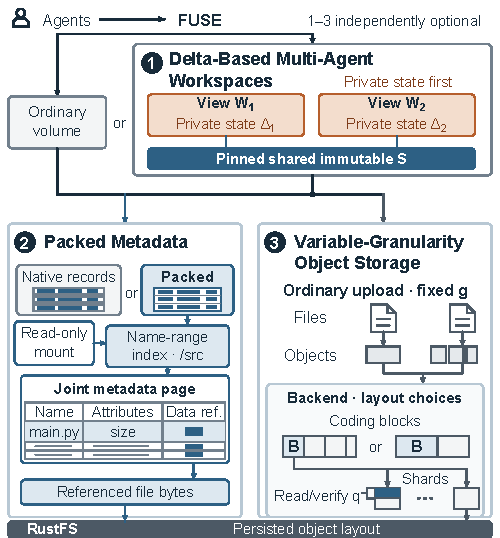
\includegraphics[width=\columnwidth]{figures/system-architecture-editable.pdf}

\caption{Three optional, composable mechanisms.
The metadata example stores file bytes separately.
In ordinary uploads, each raw block forms an object after applicable
compression/framing. Matching $U_1/O_p$ ports use separate upload contracts.
Dashed $B$ hints are optional; backends persist effective layouts.
Integration limits appear in Section~\ref{sec:implementation}.}
\label{fig:overview}
\end{figure}

Writes introduce two distinct visibility boundaries. A dirty buffer can
serve this client's reads before its bytes are remotely durable.
Publishing a recoverable immutable version requires its referenced
objects to satisfy the selected persistence contract and its metadata
to be validated. Private namespace state alone does not establish that
boundary, and a local read returning new bytes does not establish it
either.

Publication also creates a lifetime obligation: workspace and reader
ownership must retain referenced metadata and payloads until they can be
reclaimed. Backend layout selection can change how an object is encoded
and read while preserving its logical identity and contents. Readers of
an existing version continue to interpret each object using its persisted
layout.

A published file version may contain application checkpoints; restoring
process memory, open handles, and execution state remains the runtime's
responsibility. The next sections develop workspace resolution, immutable
metadata access, and object formation. Section~\ref{sec:implementation}
identifies their current mount and recovery paths.

\section{Delta-Based Workspaces}
\label{sec:delta}

\subsection{Creating a view and resolving names}

A workspace binds an immutable lower $S$ and private writable upper
$\Delta_i$, yielding $W_i=\operatorname{Resolve}(S,\Delta_i)$. Creation
registers the base identity and private control state without copying the
complete metadata tree. The catalog path identifies the base by layer,
sealed version, and root hash; a packed lower additionally binds its
authenticated manifest. Binding validation, ownership records, and mount
preparation still contribute to creation cost.

A name lookup first consults the private record, which distinguishes a
present entry, an explicit deletion, and absence. For parent directory
$d$ and name $n$, let $H_i(d,n)$ indicate that an applicable rule blocks
inheritance of that lower name. Then
\begin{equation}
R_i(d,n)=
\begin{cases}
e, & \Delta_i(d,n)=\operatorname{Present}(e),\\
\bot, & \Delta_i(d,n)=\operatorname{Whiteout},\\
\bot, & \Delta_i(d,n)=\operatorname{Absent}\land H_i(d,n),\\
R_S(d,n), & \Delta_i(d,n)=\operatorname{Absent}\land\neg H_i(d,n).
\end{cases}
\end{equation}
Here $\bot$ denotes absence. $H_i$ covers directory-opacity or other
lower-inheritance rules without hiding a present upper entry. A whiteout
terminates lookup; deleting an inherited name must preserve this marker,
since merely removing a private record could expose the lower name again.

Directory enumeration applies the same precedence to each name, removes
duplicates, and returns attributes of the visible inode. The catalog-backed
buffered path and a direct-I/O workspace path both retain an inherited file's
inode number when materializing private attributes or mappings. Updates
through one hard-link alias therefore remain visible through the others.

The direct-I/O path uses a transactional private namespace. Rename locks
participating inodes in number order, validates the observed rows and writer
authority, then atomically commits the source
whiteout, destination binding, and affected inode and parent records.
Its namespace reads validate an operation-local view and retry conflicts:
a successful read can observe either side of a concurrent rename, but
not its partially updated rows. Separate calls may straddle that commit.
The catalog-backed buffered path instead serializes local mutations and
uses version-guarded catalog transactions. These mechanisms do not establish a
snapshot across multiple system calls; entry-specific caching and runtime
bounds remain as described in Section~\ref{sec:implementation}.

\subsection{Resolving overwrites and truncation}

An overwrite changes which bytes a file range references. The buffered
path records private data extents alongside namespace and inode changes.
The direct-I/O path represents each changed logical chunk by a normalized
map with explicit spans of upper data, lower references, or zeros. These
respectively identify newly stored bytes, inherited bytes in $S$, and holes.
An explicit map covers its applicable range completely; an uncovered
interval is not an implicit lower reference.

A short overwrite replaces its mapped interval while preserving lower
references elsewhere. In this path, truncation first commits the reduced size,
a nonincreasing lower-visible boundary, and a cleanup intent. Cleanup
replaces discarded spans, including existing upper data, with zero spans;
subsequent extension completes pending cleanup before changing the size.
For example, writing upper bytes at $[6,10)$, shrinking to 7, then extending
to 34 must yield zeros at $[7,34)$. Lower-visible size alone would not
invalidate the old upper bytes. These steps describe the direct-I/O path;
other mounts retain their own update protocols. Object formation
remains separate: a short logical write need not produce a short object.

The buffered client's dirty overlay makes its bytes readable before writeback
completes. If local dirty data covers
$[4,8)$ KiB, a read of $[2,10)$ KiB combines two committed 2 KiB ranges
with the dirty 4 KiB range. A buffered workspace can use both this overlay
and persistent private mappings; local read-your-writes alone establishes
neither remote durability nor a published recovery point.

\subsection{Publishing and retaining a version}

The direct-I/O workspace uploads an object durably before publishing its
mapping. The ordinary buffered path defaults to upload-before-commit and
offers explicitly selected commit-before-upload mode, which can expose
mappings before their objects
are remotely available.
Preparing a recoverable version therefore requires draining and validating
referenced objects even when local reads already return new data.

A worker handoff requires application checkpoints, stopping new source
writes, and making required payloads and metadata durable before publishing
the immutable version. The destination binds that version and acquires
write authority; lease and generation checks reject stale writers.
Applications restore execution state and reopen files from this recovery
point. Section~\ref{sec:implementation} distinguishes implemented lifecycle
components from connected recovery paths.

Publication must preserve prior versions still held by workspaces or readers.
Reclamation separates those references from abandoned construction
objects. For one shared baseline, live logical metadata obeys
\begin{equation}
M_{\mathrm{live\text{-}meta}}=M_S+\sum_i M_{\Delta_i}+M_{\mathrm{control}}.
\end{equation}
$M_S$ counts the shared metadata once; $M_{\Delta_i}$ counts private names,
attributes, deletion records, and mappings; $M_{\mathrm{control}}$ counts
disjoint binding and ownership records. Upper payload, encoding and
checksum overhead, unreclaimed objects, and caches belong to separate
physical accounting. Complete private records and mappings grow with
modification and deletion; comparison with materialized workspaces must
match visibility and durability contracts.

\section{Packed Metadata}
\label{sec:packed}

\subsection{Organizing immutable records for reuse}

Once a source view is fixed, its metadata no longer needs to accommodate
in-place record updates. The producer can organize records for retrieval,
build their indexes once, and let readers reuse that organization for the
version's lifetime. Packed metadata applies this principle to directory
entries, common attributes, and file-data locators, placing related records
in bounded pages on object storage. It moves organization work to
construction while retaining demand-driven access to the resulting snapshot.

The snapshot describes a selected subtree and can directly back a standalone
read-only mount. It can also serve as the optional immutable lower of a
delta-based workspace, where the workspace mechanism resolves private
changes before consulting inherited records. This choice of representation
does not require a particular backend layout; native catalog records remain
an alternative lower representation.

A logical read group covers one parent directory and a range of raw entry
names in byte order. Its GroupMeta page co-locates each entry with common
attributes and data locators, so a name lookup can supply information needed
by subsequent attribute and data operations. Neighboring names may reuse
the same page. The raw page is bounded at 256 KiB, while a physical container
may hold several groups. This separates the unit of metadata organization
from the object that stores it. Range indexes route requests to these groups;
their height depends on page capacity and record count, rather than on
the source directory tree's depth.

\begin{figure}[t]
\centering
\begin{tikzpicture}[
  b/.style={draw,rounded corners=2pt,align=center,text width=6.5cm,minimum height=0.56cm,font=\small,fill=black!3},
  a/.style={-{Latex[length=1.7mm]},semithick}
]
\node[b] (root) {Pinned manifest and authenticated roots};
\node[b,below=0.35cm of root] (index) {Paged directory-name index\\$(\text{parent},\text{raw-name interval})$};
\node[b,below=0.35cm of index] (group) {GroupMeta page\\entry $+$ common attributes $+$ data locator};
\node[b,below=0.35cm of group] (frame) {Packed frame descriptor\\container offset, length, content verification};
\node[b,below=0.35cm of frame] (data) {Payload range read and verification};
\draw[a] (root) -- (index);
\draw[a] (index) -- (group);
\draw[a] (group) -- (frame);
\draw[a] (frame) -- (data);
\end{tikzpicture}

\caption{Representative packed-snapshot lookup/read path.
A name lookup supplies joint metadata and a data locator; reading referenced
data resolves authenticated descriptors before fetching and verifying payload ranges.}
\label{fig:packed}
\end{figure}

\subsection{Querying a pinned snapshot}

A reader pins a manifest identity and starts from its authenticated index
roots. For \code{lookup(parent,name)}, the directory-name index identifies
the group covering the key. The reader resolves its container reference and
fetches the GroupMeta byte range. It verifies the stored-byte digest before
decoding, then checks the decoded entry count and name boundaries against
the authenticated group reference. The matching record supplies the inode,
common attributes, and data locator (Figure~\ref{fig:packed}).

The query input determines which index is needed. Direct \code{getattr}
can obtain common attributes through an inode index, while enumeration
traverses ordered name ranges and uses counted indexes for directory-ordinal
navigation. A file read returns inline contents or follows a data locator
to an authenticated descriptor, fetches the referenced payload range, and
verifies it. Packed data frames define snapshot-level access and integrity
units; the backend serves these object requests using its own persisted
layout.

For supported snapshot queries, these paths obtain names, attributes, and
data locations without consulting per-file records in the mutable metadata
database. A writable workspace still performs its private upper checks and
control operations separately. Lower-query independence thus describes
where inherited records are obtained, while leaving workspace mutation and
lifetime coordination to their own protocols.

\subsection{Preserving identity and authenticated results}

Every returned record or payload must be connected by authenticated
references to the pinned manifest. Checking a fetched page's digest is one
part of this rule; checking its declared key boundaries and decoded contents
also prevents accepting the wrong records for a query. A missing referenced
object or failed authentication is an error, not evidence that a requested
name is absent.

The same pinned identity governs reuse. Authenticated pages and resolved
records remain valid for that version without tracking per-record updates.
Publishing a later version therefore does not change the records seen by
an existing reader. Caches can reuse these results, but their effectiveness
depends on locality: a cold lookup may traverse several index pages, and a
data read may require descriptor and payload requests beyond the metadata
page. Co-location provides an opportunity to reuse fetched information,
rather than a fixed number of GETs per operation.

\subsection{Publication, lifetime, and amortization}

Construction needs a consistent source view, established through a snapshot
or an explicit validation protocol. The producer groups records, uploads
their referenced objects, and produces the indexed manifest. Output
immutability alone cannot establish source consistency. Before publishing
a binding, the selected protocol must establish that its required objects
are durable and valid; producing a manifest and publishing its reference are
separate events. Readers retain their pinned versions, and reclamation must
preserve objects still required by retained versions or readers. Rebuilding
creates another version; ordinary file close does not rebuild a snapshot.

The access benefit depends on how much of each fetched page is useful.
Repeated nearby lookups can reuse joint metadata, whereas isolated lookups
may transfer records they never consume. Inlining file contents, compressing
pages, and co-packing payload regions also affect transfers, decoding, and
cache use. Their costs must be separated from the effect of metadata
co-location.

Construction, validation, publication, rebuilding, and reclamation all enter
the cost comparison. For one published version's lifecycle and $K$ uses,
we will measure each additive resource metric $c$ as
\begin{equation}
C_c(K)=C_{c,\mathrm{build}}+C_{c,\mathrm{publish}}
       +\sum_{i=1}^{K}C_{c,i}+C_{c,\mathrm{reclaim}}.
\end{equation}
The per-use terms include setup and access work for the chosen reuse unit;
construction and publication terms include their required validation.
CPU-seconds, transferred bytes, and monetary cost are separate metrics;
concurrent task wall-clock times are not summed into a batch makespan.
For repeated rebuilding, costs are accumulated over the resulting versions,
with shared work charged only once.
Reuse pays for construction only when the accumulated access savings exceed
these costs. Frequent rebuilding, weak name locality, or expensive cold
index walks can erase the benefit.

Immutable object-backed metadata already has strong
precedents~\cite{deltafs2021,cvmfs2011,nydus_rafs}. We will compare the joint
layout with immutable sorted-KV records at equal content and cache budgets,
and with compatible demand-loaded immutable-image systems. Standalone
read-only and workspace-lower use are separate comparisons. The sorted-KV
control tests layout organization and is not a reproduction of DeltaFS.

\section{Variable-Granularity Object Storage}
\label{sec:layout}

A file read names a logical byte range, but its cost depends on the objects
containing that range, the bytes fetched, and the storage units verified.
Large objects can reduce request count for sequential access while increasing
the work needed to serve a partial read. \sysname{} therefore separates
client object formation from backend encoding and verification. The
connection between them is the finalized object, whose length becomes known
after assembly, applicable compression, and framing.

\subsection{From file ranges to objects}

The ordinary data path maps file offsets to logical chunks and resolves
the visible slices within each chunk. A chunk is an addressing range;
slices identify the written content that supplies its visible intervals.
The uploader partitions each slice's data using the configured client
block size $g$ and stores the resulting blocks under the slice identity
and block index. A 10 MiB slice with $g=4\MiB$, for example, can produce
raw blocks of 4, 4, and 2 MiB.

Compression, headers, and framing then determine each object's finalized
upload length $L_o$. Thus $g$ controls the partition of the slice, whereas
$L_o$ describes the bytes actually uploaded. Flush boundaries and partial
writes affect which slices and objects form, and a short tail need not
occupy a full block. When reading, the client uses the same geometry to
translate a visible slice interval into object references and offsets.
A new slice can replace one interval while untouched intervals continue
to reference older objects; the replacement need not rewrite the complete
old object.

The ordinary path defaults to 64 MiB chunks and $g=4\MiB$, with a chunk
size that is a nonzero multiple of $g$. This is a fixed configuration.
The proposed 1/4/8/16 MiB choices define an object-formation design space,
not an implemented controller that selects sizes from access behavior.
Because readers reconstruct block addresses from the configured geometry,
changing $g$ for existing data requires a compatible representation or
migration.

\subsection{Mapping objects to backend storage}

Once $L_o$ is known, a compatible RustFS research backend can use it to
inform a separate layout decision. Let $B$ denote the backend's
erasure-coding block size. The client may request $B$ through an
encoding-block-size hint $h(L_o)$, without changing $g$ or multipart part
sizes. The backend validates the request under its compatibility and
eligibility rules and persists the effective $B$. Omitting a hint retains
default selection. Multipart initiation uses the complete object's length,
and retries retain that object's decision.

The current interface supports fixed hints of 64 KiB, 256 KiB, 1 MiB, and
4 MiB. Its automatic hint policy omits the hint for $L_o\leq1\MiB$ and
requests $B=1\MiB$ otherwise. This rule acts on the formed object; it does
not select the client block size. The backend also defaults to $B=1\MiB$,
so automatic and default settings need not produce different layouts.

The physical verification/read quantum $q$ determines how much shard data
must be verified together.
For $d$ data shards and $p$ parity shards, let $s$ be one complete stripe's
logical shard size. A separately enabled backend policy can select a
physical verification/read quantum for eligible new framing subject to
\begin{equation}
q\mid s, \qquad qd\mid B.
\end{equation}
These are admission constraints for the new framing, preserving stripe
alignment while permitting smaller verification units. Both hint admission
and new $q$ framing have their own compatibility gates. Reads and healing
use persisted object geometry even after write settings change.

\subsection{From an object range to physical work}

Object size alone does not determine the bytes fetched for a file read.
Range GET can retrieve part of an object when its format permits independent
access. The ordinary store supports page-aligned range reads for eligible
small requests; compressed blocks or a whole-object fetch policy can require
larger transfers. A packed frame provides a decoding and integrity boundary
inside a snapshot object, distinct from both the client block size $g$ and
the backend quantum $q$. Caching and concurrent-read coalescing determine
which of these requests reach the backend.

The backend maps the resulting object range into shard intervals.
For a shard interval $[a,a+\ell)$, with $a\geq0$, $\ell>0$, and $q>0$,
the number of verification/read quanta intersected is
\begin{equation}
n_q(a,\ell)=
\left\lceil\frac{a+\ell}{q}\right\rceil-
\left\lfloor\frac{a}{q}\right\rfloor.
\end{equation}
Ignoring tails and batching, the covered data is approximately $n_q q$
plus checksums, summed over shards actually read. The application request
cannot be substituted directly for $\ell$: the client range, compression,
and coding determine that interval. Smaller $q$ can reduce over-read while
increasing checksum overhead. For fixed $(d,p)$, the nominal redundancy
remains $(d+p)/d$; a large $B$ does not imply a fully padded tail stripe.

\subsection{Costs and scope}

The tradeoff in $g$ is visible even before backend encoding.
Table~\ref{tab:object-granularity} considers one uncompressed 64 MiB slice
starting at file offset zero and a read of $[10,12)\MiB$. Increasing $g$
reduces the number of objects in the slice, but increases bytes fetched
for this read if complete objects must be obtained. These are arithmetic
examples, not measurements or a policy recommendation.

\begin{table}[t]
\centering
\begin{tabular}{rrr}
\toprule
$g$ & Object count & \shortstack{Whole-object\\bytes fetched}\\
\midrule
1 MiB & 64 & 2 MiB\\
4 MiB & 16 & 4 MiB\\
8 MiB & 8 & 8 MiB\\
16 MiB & 4 & 16 MiB\\
\bottomrule
\end{tabular}
\caption{Idealized object formation and a 2 MiB partial read. The last
column assumes complete fetches of the intersecting objects, with no cache
hits or compression and ignoring framing overhead; it does not describe
every range-read path.}
\label{tab:object-granularity}
\end{table}

These layers require separate cost accounting. Network read amplification
compares object response bytes with application bytes served; upload
amplification compares uploaded bytes with application bytes written;
physical read amplification compares storage-device bytes with application
bytes served. Request counts, compression work, and cache occupancy capture
additional costs. Compaction, retries, and accumulated short slices can
increase upload work, so smaller objects do not guarantee lower write
amplification. Similarly, whole-object fetching can prevent a smaller $q$
from reducing the work generated by a partial application read.

The mechanism applies to an ordinary flat volume without delta-based
workspaces or Packed Metadata. Either of those mechanisms can also retain
fixed client geometry and default backend layouts. Their composition
changes the referenced objects and access patterns, while snapshot
producers and workspace upper writers retain their own object formats and
upload contracts. Section~\ref{sec:implementation} describes these path
boundaries and the ordinary client's coupling of enabled hints with
whole-object fetch and cache policy. That coupling must be separated from
backend geometry when attributing a measured effect to $B$ or $q$.

\section{Implementation Boundaries}
\label{sec:implementation}

The implementation connects the mechanisms through several access paths.
Their differences affect both guarantees and performance attribution.
The following boundaries come from source inspection; the companion
record identifies the inspected revisions, while runtime and failure
validation remain part of the evaluation plan.

\subsection{Buffered and direct access}

An ordinary volume resolves mutable metadata and sends file data through
buffered caching and writeback. A workspace can reuse this path while
replacing metadata lookup with private-state resolution over a sealed
catalog or packed lower. A standalone snapshot reader instead provides
read-only access without constructing a private upper. Its metadata cache
is separate from payload caching; the current read-only path does not
admit configurable payload-cache or prefetch budgets.

A second workspace implementation stores current private namespace and
mapping records transactionally and uses a dedicated direct-I/O adapter.
This is the concrete namespace and truncation path described in
Section~\ref{sec:delta}. It bypasses ordinary buffered writeback and
metadata TTL caching. Its operation sizes, complete-directory enumeration,
and live ownership set have admission bounds. It currently supports
newly created workspaces, without process-crash takeover. These limits
belong to that path, rather than the logical workspace model or every mount.

The direct path authenticates an entire upper object before returning a
subrange. Thus a smaller backend verification unit need not reduce work
for a short application read. Comparing this path with a buffered volume
changes cache and fetch behavior as well as workspace representation;
an ablation must retain one access path or control those changes explicitly.

\subsection{Publication and recovery}

Snapshot publication validates uploaded objects before installing the
lower binding and acquiring reader ownership. Recovering a binding also
requires generation and lease checks: knowing a manifest's identity does
not grant authority to resume writes. One connected recovery path reuses
the same persistent storage allocation and checks its worker identity and
scoped metadata authority. It does not provide arbitrary-worker migration.

Catalog lifecycle operations encode quiescence, object verification,
retention, and atomic version transitions. Connecting these operations
to worker handoff still requires runtime orchestration. The recovery
target is a published file state; applications must checkpoint execution
state and reopen tools separately. Source-level lifecycle operations
therefore do not by themselves demonstrate end-to-end recovery.

\subsection{Object formation and layout admission}

The ordinary uploader partitions slices using fixed volume geometry,
defaulting to $g=4\MiB$ within 64 MiB chunks. Readers use the same geometry;
an incompatible configuration is rejected. The proposed 1/4/8/16 MiB
settings expose a design space, not an adaptive sizing policy.

Backend hints are optional and require both client support and compatible
storage servers. Hint admission and new verification framing have separate
enable and fleet-compatibility gates, disabled by default. The backend
checks eligible writes and persists their effective layouts, which govern
later reads and repair. Changing admission settings does not re-encode
existing objects.

Uploader coverage matters. The ordinary uploader propagates hints; direct
workspace writes and the current snapshot producer use default settings.
Extending them must preserve conditional object creation and rejection of
conflicting writes. Direct workspace uploads also form objects from write
fragments, rather than ordinary buffered blocks, and cap those fragments
at the automatic policy's no-hint threshold.

That policy omits hints for $L_o\leq1\MiB$ and requests $B=1\MiB$
otherwise; the inspected backend already defaults to $B=1\MiB$.
Enabling hints can therefore leave the stored layout unchanged while
changing client fetch and cache policy. Experiments must record actual
$(g,L_o,B,q)$ and physical work, and separate those client effects from
backend geometry. These integration restrictions constrain current
comparisons without making any of the three mechanisms mandatory.

\section{Evaluation Plan}
\label{sec:evaluation}

The evaluation will test when each mechanism repays its cost, whether
composition adds value, and whether those effects matter for complete
agent tasks. Table~\ref{tab:rqs} organizes these questions; the companion
matrix specifies experiments E00--E16 and their instruments and admission
checks. All system comparisons below are planned. The completed FUSE
study in Section~\ref{sec:agent-observations} supplies request-structure
evidence for RQ1, while cross-task sharing, locality, and system performance
remain to be measured.

\begin{table*}[t]
\centering
\scriptsize
\begin{tabularx}{\textwidth}{@{}p{0.65cm}p{4.6cm}Yp{1.60cm}@{}}
\toprule
RQ & Question & Primary evidence & Plan\\
\midrule
1 & Which workload properties favor shared immutable state? & Observed: per-task FUSE request mix, read/write sizes, and time variation. To measure: cross-task read-set overlap, mutation footprint, locality, and tool-phase-labelled access. & E01--E02\\
2 & When do delta-based workspaces reduce workspace cost? & Time to usable workspace, private metadata, modification and lifecycle costs & E03--E04\\
3 & What does packed metadata save, and at what cost? & Metadata-KV calls, object requests/bytes, latency, cache effects, construction amortization & E05--E07\\
4 & What changes with $g$, $(B,q)$, and client read policy? & Object formation, persisted geometry, physical bytes, verification/EC CPU, durable writes and repair & E08--E10\\
5 & Do the mechanisms provide additional combined value? & Legal factorial or nested comparisons under one runtime contract & E11\\
6 & Do the effects matter for complete multi-agent tasks? & Deterministic replay, live-task makespan, resource use, output-quality controls & E12--E13\\
7 & Which semantics and failure boundaries hold? & Differential operations, fault injection, integrity, reclamation and long-run resource bounds & E14--E16\\
\bottomrule
\end{tabularx}
\caption{Research questions and evidence status. RQ1 separates the observed
request-structure pilot from further measurements; the remaining rows are
planned. E00 first checks that each
configuration is connected and produces the claimed effective treatment.}
\label{tab:rqs}
\end{table*}

\subsection{Environment and baseline contracts}

The proposed primary testbed separates two clients, one metadata server,
and four RustFS storage servers on a 25 GbE network. The requested clients
have 24--32 physical cores, 128 GiB memory, independent NVMe storage, and
fixed cache allocations. The initial layout will use one drive per storage
server in a verified 2+2 set. A single-host, four-drive setup will support
earlier functional and mechanism experiments; machine-failure experiments
require the distributed testbed.

We will record processor, memory, disks, network, OS/kernel, FUSE settings,
toolchain, complete configuration, build features, immutable image digests,
and source revisions. Client object-block granularity $g$, durability,
compression, cache budget, readahead,
direct I/O, metadata TTL, inline thresholds, and backend gates are part of
the treatment definition. Larger coding geometries will be separate
experiments because they can change whether the selected $q$ is smaller than
the logical shard size.

External baselines include full copying, reflinks where supported, OverlayFS,
BranchFS, and an object-backed file system such as JuiceFS~\cite{juicefs_architecture} sharing the same
backend resources. At least one mature immutable lower, such as Nydus or
CernVM-FS, will be tested with a compatible writable layer. An immutable
sorted-KV lower with equal records and cache capacity provides a specific
layout control. A real DeltaFS comparison depends on its operation and
workflow compatibility. The sorted-KV control isolates representation
and is not a substitute for the DeltaFS system.

We will compare local workspace service separately from remote durable
service. An OverlayFS local fsync is not equivalent to remote coded-object
completion. Similarly, BranchFS's ephemeral branch uses different fsync and
commit semantics~\cite{branchfs2026}. Where a baseline needs a checkpoint to
meet the selected persistence boundary, its completion cost is included.
If equivalent semantics cannot be provided, we report separate operating
points instead of one unconditional speed ranking.

\subsection{Workload characterization}

\researchq{1} The workload study will identify the conditions under which
sharing and grouping are useful. With the agent harness and model pinned,
we will measure cross-task read-set overlap, directory locality, reuse
distance, mutation footprint, and per-task operation distributions across
navigation, editing, build/test, and cleanup. The study will retain Core
and Exploratory task strata and report each new run's request mix and
temporal bursts. Failed lookup and attribute probes will be classified
separately from I/O failures, and an
instrumentation-on/off control will quantify tracing overhead and loss.

The next capture will connect task behavior to the storage path. It must
retain paths, payloads, handle dependencies, synchronization relations,
and tool-phase boundaries for replay, and connect FUSE requests to $g$,
final uploaded lengths $L_o$, and actual client fetches. This information
is absent from aggregate counts and size histograms. It is needed to
distinguish object formation from request selection and backend processing.

The proposed expanded panel contains 20 compatible tasks each from
SWE-bench Verified, a fixed public SWE-bench Pro version~\cite{swebench_pro_v2}, and a multilingual
set informed by Multi-SWE-bench~\cite{swebench2024,multi_swebench2025}.
Exact task lists and revisions will be frozen after capability screening.
An official audit has identified limitations in using SWE-bench Verified
to measure frontier model ability~\cite{swebench_audit2026}; we use it as a
reproducible workload source and retain other task families. Filesystem
performance does not establish improved reasoning ability.

The minimum live-agent core will use 20 prespecified tasks, three systems,
and three independent repetitions at one concurrency setting: 180 runs.
The 60-task extension requires 540 runs for that same setting, before any
additional model or concurrency sweep. Pilot task duration and token use
will determine a frozen budget. Broad concurrency sweeps will first use
replay, with live experiments reserved for the prespecified conditions.

To attribute cost to task activity, the capture will distinguish six
traceable phases: (A) workspace creation and dependency discovery, (B)
repository navigation (`stat', `readdir', `open', `readlink', and small
reads), (C) edit and patch writes, (D) build and test with sequential reads
and generated files, (E) dependency installation or cleanup with create,
rename, unlink, and hard-link operations, and (F) diff, discard, or retained
workspace teardown. We will retain phase boundaries and report per-phase
and whole-task critical paths. Controlled replay will preserve paths,
payload hashes, handle lifetimes, and synchronization events; live runs
will additionally record model/tool spans. This attribution separates
provisioning from execution costs and captures namespace activity beyond
the data I/O exercised by fio.

Table~\ref{tab:agent-load} specifies the primary workload panel and the
controls needed to interpret each phase.

\begin{table*}[t]
\centering
\scriptsize
\begin{tabularx}{\textwidth}{@{}p{1.1cm}p{3.3cm}Yp{2.0cm}@{}}
\toprule
Phase & Representative operations & Treatment and baseline controls & Primary outputs\\
\midrule
A/B & fan-out, path walk, `git status', grep, metadata-only scans &
shared lower versus materialized checkout; cold/index-warm/data-warm states &
ready time, lower-KV calls, GETs, metadata P99\\
C & patch, overwrite, truncate, sparse write, fsync &
matched write-completion and cache budgets; 0.1--10\% mutation &
upper bytes, commit and drain tail, write amplification\\
D & compiler reads, test binaries, generated artifacts &
same dependency image and local build cache; sequential/random mix &
critical path, read bytes, CPU, task makespan\\
E/F & install, rename/unlink storms, retry, diff/discard &
same lifecycle and durability boundary; retain failed and timed-out runs &
whiteouts, retained objects, cleanup lag, success\\
\bottomrule
\end{tabularx}
\caption{Agent file-system load panel. The table defines the workload
phases; it does not assert that every agent task exercises them equally.}
\label{tab:agent-load}
\end{table*}

\subsection{Individual mechanisms and lifecycle costs}

\researchq{2} Workspace experiments will test whether sharing reduces
provisioning and retained state after private modifications and cleanup
are included. They will vary lower size, workspace count, and
modification fraction. Initial values are $10^4$--$10^6$ files, 1--128
workspaces, and 0--50\% modified files. We measure control-plane return,
mount readiness, first navigation, and first durable edit separately.
Prepositioned and cold-staged baselines are separate cases. Churn experiments
add deletion, rename, truncation, and repeated lifecycles, subject to the
selected implementation's ownership and cleanup support.

\researchq{3} Packing experiments will test whether metadata access savings
repay snapshot construction and maintenance. They will compare mutable per-file KV,
immutable sorted-KV, and the packed layout using equivalent values and
cache budgets. Standalone read-only access tests the packed representation
independently of delta-based workspaces; workspace experiments then compare
the same representations as alternative lowers. Both include positive and
negative lookup, direct getattr, enumeration,
lookup-plus-read, deep paths, and wide directories. The snapshot reader's
large-directory study is separated from the Entity bridge's 4,096-entry
limit. We count upper/control/lower KV requests independently, as well as
index, GroupMeta, descriptor, and payload object requests and bytes.

Cold-client, index-warm, metadata-warm, and data-warm states are explicitly
defined; backend page-cache state is another variable. Unsupported
payload-cache controls are not treated as available flags. Snapshot
construction, publication, rebuilding, and reclamation enter each resource
accounting metric. We report a break-even reuse count only if the measured
net benefit per reuse is positive, with the reuse unit fixed for each
standalone or workspace experiment.

\researchq{4} Object-granularity experiments will separate the effects of
object formation, client fetching, and backend processing. A backend-only
study will first hold the S3 request stream fixed. Object sizes cross inline,
1 MiB, encoding-block, and
multipart boundaries. $B$ settings include default, the current automatic hint
policy, and the four supported fixed values. $q$ settings are legacy or the implemented
selector, grouped by \emph{persisted} geometry. If automatic and default
produce the same $(B,q)$, they are a no-treatment control, not evidence for a
benefit from the automatic hint policy.

The file-system study adds $g$ as a separate object-formation factor. A
controlled sweep holds the logical write stream constant and records final
object lengths $L_o$, object counts, and uploaded bytes, including compression,
headers, and tails. It first holds backend geometry fixed, so changes caused
by forming different objects are not attributed to $B$ or $q$. Subsequent
comparisons cross these factors only where the selected upload path supports
them; a fixed configuration does not establish an automatic selection policy.
The ordinary client's range-read threshold scales with $g$. A causal sweep
must hold the absolute threshold constant where supported, or expose its
change as a coupled client-policy factor.

Reads vary length, alignment, crossing of encoding-block and $q$-interval
boundaries, and healthy versus degraded state. The primary measurements are physical data/parity
read bytes, checksum work, EC CPU, HTTP payload, request counts, and latency.
Client range-read and whole-object fetch policies are then separated while keeping
cache admission and coalescing constant or exposing them as additional
factors. Upper and lower results are separate because their integrity
and upload paths differ.

Writes include append, overwrite, tails, multipart retry, and frequent
durability requests. We record accepted writes, staging, remote completion,
metadata commit, and drained background debt. Repair experiments measure
read/write/network work and interference with healthy requests. The paper
will claim lower write amplification only if these measurements support
it; a read benefit can coexist with increased checksum or write cost.

\subsection{Composition and complete agent execution}

\researchq{5} Composition experiments will ask whether combining mechanisms
changes their individual effects. Each comparison must retain one runtime
contract: switching from a buffered ordinary volume to a direct-I/O Entity
mount also changes caching and writeback. We will implement or validate
matched controls for complete metadata materialization versus shared lower
state, metadata representation, $g$, and backend geometry. Client read
policy will be held constant or varied as an explicit factor.

The experiment structure will follow supported configurations. Packing
will first be tested in standalone read-only use, then as an alternative
workspace lower. Fully crossed comparisons will include only combinations
that can be constructed under the same runtime contract. Where an entry
wires a treatment only within one workspace path, that comparison will be
nested within the runtime. For full crossings, interactions in task-level
log latency will test whether combined effects differ from the individual
component effects.

\researchq{6} Complete-task experiments will connect mechanism effects to
agent execution. Deterministic replay will isolate storage behavior by
freezing tool inputs, write contents, and dependencies, while preserving
file-tree and output checks. A FUSE log containing only inode IDs and
request lengths is not necessarily replayable; paths, handle lifetimes,
payload references, initial state, and ordering must be recovered or
recaptured. Arrival-driven and closed-loop replay are reported separately.

Live AX/DSH experiments keep the task, model identifier, prompt, tools,
token/time budgets, and concurrency policy fixed. Mount probes must verify
that workspaces and subprocesses reach the intended file system rather than
a fallback directory. We measure batch makespan, tasks per hour,
provisioning, resource use, and the traced storage critical path. Model
waiting and I/O can overlap, so their durations cannot simply be added.
Output correctness is checked with the task harness; an exit code of zero
is not a resolved issue.

\subsection{Correctness, failures, and analysis}

\researchq{7} Correctness experiments will test the view and persistence
contracts on which the performance comparisons depend. Differential and
known-answer tests will cover whiteouts, same-name
recreation, lower-file modifications, truncate/extend, holes, links,
rename-overwrite, open-unlink-read, and cross-workspace visibility within
the supported contract. Fault injection targets object upload, manifest
and binding publication, mapping commit, process restart, missing objects,
frame corruption, and repair interruption. Fresh-only Entity behavior is
reported as such; reopen or crash-takeover experiments require a completed
runtime extension. Fail-closed behavior is distinct from successful recovery.

Long runs cover multiple cache and cleanup cycles and track tail latency,
memory, open descriptors, owners, pending uploads, retained objects, and
reclamation backlog. Background publishing or repair is added only where
the selected runtime supports it. High mutation, poor locality, frequent
snapshot rebuilding, and large sequential reads are explicit boundary
workloads, not exclusions from the evaluation.

\paragraph{Analysis and completion accounting.}
The independent unit is a run or a task, not each of its millions of
requests. Initial plans use at least ten independent microbenchmark blocks
and three live repeats per selected task; the formal sample sizes are
frozen after a variance pilot. Conditions are interleaved in randomized
host/time blocks. We report absolute effects, paired ratios, and 95\%
task- or repository-clustered bootstrap intervals. Repeated task outcomes
are not treated as independent binary pairs.

For live speed comparisons, the primary endpoint includes all assigned
tasks under the same deadline; failed and timed-out attempts remain in the
throughput and completion accounting. Completed-only latency is secondary
and accompanied by success rates and failure causes. Early failures do not
count as fast completions. This protocol prevents storage behavior or model
failures from creating an apparent speedup through selective omission.

\section{Related Work and Scope}
\label{sec:related}

\paragraph{Workspaces and agent-native file systems.}
OverlayFS provides layered namespaces with a private upper and shared
lower~\cite{overlayfs}. BranchFS applies copy-on-write branch contexts to
agentic exploration, with a commit/abort lifecycle described through a
workshop prototype and a proposed kernel abstraction~\cite{branchfs2026}.
YoloFS addresses visibility and control over agent effects through staging,
snapshots, and permissions~\cite{yolofs2026}; AgentFS documents a file-system
and tool-state abstraction for agents~\cite{agentfs2025}. These systems
establish workspace and agent-control mechanisms on which the present
problem builds. \sys focuses on serving private views through remote
metadata and object access. Process isolation, user approval, and the
commit semantics of other agent systems remain separate concerns.

Table~\ref{tab:comparison} identifies the comparison axes. Its last column
states the boundary to test against each baseline under matched persistence
and cache budgets; it reports no measured advantage.

\begin{table*}[t]
\centering
\scriptsize
\begin{tabularx}{\textwidth}{@{}p{1.60cm}p{1.95cm}p{2.15cm}p{2.0cm}Y@{}}
\toprule
System & Shared baseline & Private view & Remote metadata/data & Boundary tested in this work\\
\midrule
OverlayFS & local lower tree & kernel upper/copy-up & none by itself & remote immutable lower, explicit object reads, and durable upper\\
DeltaFS & immutable logs and manifests & per-job namespace & object store plus registry & current-value upper, directory-oriented pages, and online POSIX lookup\\
BranchFS & local COW branch context & branch commit/abort & prototype-local & remote persistence and multi-client lower sharing\\
CVMFS/Nydus & lazy immutable catalog/image & requires an external upper & cached objects/blobs & writable workspace semantics and metadata/data locator co-location\\
JuiceFS & chunk/slice/block volume & shared mutable POSIX view & object store plus KV & frozen metadata access, object formation at $g$, and persisted $(B,q)$ layout\\
\sys & native or packed baseline & optional private delta & objects plus metadata/control KV & separate and combined effects of view composition, packing, and object layout\\
\bottomrule
\end{tabularx}
\caption{Comparison axes used to choose baselines. Existing systems already
provide individual mechanisms; the opportunity examined here is their
independent use and optional composition for remote agent workloads.}
\label{tab:comparison}
\end{table*}

\paragraph{Namespace and metadata organization.}
TableFS, IndexFS, LocoFS, and InfiniFS organize, partition, and cache
metadata to change the work required by file-system
operations~\cite{tablefs2013,indexfs2014,locofs2017,infinifs2022}.
Recent systems also study hierarchical object metadata and distributed
update coordination~\cite{mantle2025,switchfs2026}. Their access paths make
record layout, batching, and cache reuse relevant comparison criteria:
a metadata service need not issue one remote request per file operation.

DeltaFS is a particularly close conceptual predecessor. It uses private
namespaces and immutable mutation logs over shared storage, with selective
composition of prior state~\cite{deltafs2021}. \sys builds on the separation
of shared state and private changes, and examines the metadata access units
used to serve a file view. Packed Metadata places common attributes and
data locators in indexed, bounded groups. It can serve a standalone
read-only view or the immutable lower of an online private workspace,
while the workspace contract also admits a native metadata lower. This
separation permits comparing the representation independently of view
composition, then measuring the cost of combining them.

\paragraph{Immutable distribution and storage backends.}
CernVM-FS provides demand-driven software distribution with indexed
catalogs, while Nydus describes metadata/data organization for lazy
image access~\cite{cvmfs2011,nydus_rafs}. Slacker and DADI also address
image distribution and startup costs~\cite{slacker2016,dadi2020}.
These systems supply close comparisons for on-demand access to an
immutable baseline. The distinguishing questions concern how records and
data locators are obtained, which fetched units can be reused, and how
construction and staging costs are amortized. The planned comparisons
cover both standalone read-only access and reuse beneath writable views.

Distributed systems such as Ceph and Tectonic separate aspects of metadata
and data services~\cite{ceph2006,tectonic2021}. Erasure-coded storage research considers
repair cost, changing redundancy over a file's lifetime, and the relation
between data placement and redundancy~\cite{azureec2012,morph2024,okapi2025}.
Okapi's separation of striping and redundancy grouping is different from
our $(B,q)$ distinction, although both motivate making coupled decisions
explicit. Client block granularity $g$ additionally determines how file
data forms objects; it is distinct from backend coding and physical
verification granularity. Our comparisons hold the code rate fixed and
separate object counts, checksums, tails, and repair work. Reducing a block
size can change these costs without changing the nominal redundancy ratio.
The same distinction applies to ordinary volumes, workspace data, and
packed snapshots where the selected object path supports layout selection.

\paragraph{Scope and unresolved evidence.}
The design targets three conditions: sufficient unchanged state to reuse
a baseline, sufficient reuse of immutable records to repay packing, and
an access pattern for which a different object or backend unit reduces
total storage work. These conditions need not occur together. Poor name
locality, high mutation, or rapid snapshot churn may favor a native
metadata path even when a different object layout is useful. The current
entry points and lifecycle support further bound the combinations that can
be tested (Section~\ref{sec:implementation}). Establishing each mechanism's
useful region and any additional value from composition remains the
purpose of the evaluation plan.

\section{Conclusion}

\sys separates a shared version's identity from the metadata and object
units used to serve it. Its workspace, packed-metadata, and object-layout
mechanisms expose different opportunities to reduce storage work, subject
to visibility, publication, and lifetime constraints. The eight-task FUSE
study characterizes request structure, and the source audit identifies
available runtime paths. The remaining evaluation must test whether
metadata-database relief and access savings repay lifecycle costs under
matched contracts, and how these affect branching, migration, and concurrent
tasks. The planned external comparison uses JuiceFS. The present evidence
characterizes the workload and implementation
scope; it does not establish a system-performance gain.


\label{page:bodyend}
\bibliographystyle{plain}
\bibliography{references}
\end{document}
